\documentclass[10pt]{article}
\usepackage[utf8]{inputenc}
\usepackage[spanish]{babel}
\usepackage[T1]{fontenc}
\usepackage{amsfonts}
\usepackage{amsmath}
\usepackage{mhchem}
\usepackage{amssymb}
\usepackage{geometry}
\usepackage{graphicx}
\usepackage{stmaryrd}
\usepackage[export]{adjustbox}
\graphicspath{ {./images/} }
\usepackage{bbold}


\title {\textbf{Un algoritmo de dos fases para reconocer actividades humanas en el contexto de la Industria 4.0 y los procesos impulsados por el ser humano }}


\author{Borja Bordel $^{1}$, Ramón Alcarria ${ }^{1}$, Diego Sánchez-de-Rivera ${ }^{1}$\\
${ }^{1}$ Universidad Politécnica de Madrid,\\
Madrid, España\\
bbordel@dit.upm.es, ramon.alcarria@upm.es, diegosanchez@dit.upm.es}
\date{}


\begin{document}
\maketitle


\begin{abstract}
 Los futuros sistemas industriales, una revolución conocida como Industria 4.0, están previstos para integrar a las personas en el mundo cibernético como prosumidores (proveedores de servicios y consumidores). En este contexto, los procesos impulsados por humanos aparecen como una realidad esencial y se requieren instrumentos para crear bucles de información de retroalimentación entre el subsistema social (personas) y el subsistema cibernético (componentes tecnológicos). Aunque se han propuesto muchos instrumentos diferentes, hoy en día las técnicas de reconocimiento de patrones son las más prometedoras. Sin embargo, estas soluciones presentan algunos problemas pendientes importantes. Por ejemplo, dependen del hardware seleccionado para adquirir información de los usuarios; o presentan un límite en la precisión del proceso de reconocimiento. Para abordar esta situación, en este trabajo se propone un algoritmo de dos fases para integrar personas en los sistemas de la Industria 4. 0 y en los procesos impulsados por humanos. El algoritmo define acciones complejas como composiciones de movimientos simples. Las acciones complejas se reconocen utilizando modelos ocultos de Markov y los movimientos simples se reconocen utilizando Dynamic Time Warping. De esa manera, solo los movimientos dependen de los dispositivos de hardware empleados para capturar información, y la precisión del reconocimiento de acciones complejas aumenta considerablemente. También se realiza una validación experimental real para evaluar y comparar el rendimiento de la solución propuesta. Además, la precisión del reconocimiento de acciones complejas aumenta considerablemente.

\end{abstract}

Palabras clave: Industria 4.0; reconocimiento de patrones; Dynamic Time Warping; Inteligencia artificial; Modelos ocultos de Markov(HMM).

\section{Introducción}
La Industria 4.0 [1] se refiere al uso de Sistemas Ciber-Físicos (uniones de procesos físicos y cibernéticos) [2] como componente tecnológico principal en futuras soluciones digitales, principalmente (pero no solo) en escenarios industriales. Típicamente, la digitalización ha provocado, al final, la sustitución de los mecanismos tradicionales de trabajo por nuevos instrumentos digitales. Por ejemplo, los trabajadores de las cadenas de montaje fueron sustituidos por robots durante la tercera revolución industrial. 
\newline

Sin embargo, algunas aplicaciones industriales no pueden basarse en soluciones tecnológicas, siendo aún imprescindible el trabajo humano [3]. Los productos hechos a mano son un ejemplo de aplicaciones donde la presencia de obras humanas es fundamental. Estos sectores industriales, en cualquier caso, también deben integrarse en la cuarta revolución industrial. De la unión de los Sistemas Ciber-Físicos (CPS) y los humanos actuando como proveedores de servicios (obras activas), surgen los CPS humanizados [4]. En estos nuevos sistemas, se permiten procesos impulsados por humanos [5]; es decir, procesos que son conocidos, ejecutados y gestionados por personas (aunque pueden estar vigilados por mecanismos digitales). 
\newline

Para crear una integración real entre las personas y la tecnología, y mover la ejecución del proceso desde el subsistema social (humanos) al mundo cibernético (componentes de hardware y software), se necesitan técnicas para la extracción de información. Se han reportado muchas soluciones y enfoques diferentes durante los últimos años, pero hoy en día las técnicas de reconocimiento de patrones son las más prometedoras. 
\newline

El uso de Inteligencia Artificial, modelos estadísticos y otros instrumentos similares han permitido un desarrollo real e increíble de soluciones de reconocimiento de patrones, pero aún quedan algunos retos pendientes. 
\newline

En primer lugar, las técnicas de reconocimiento de patrones dependen del dispositivo de hardware subyacente para la captura de información. La estructura y el proceso de aprendizaje cambia si (por ejemplo) en lugar de acelerómetros consideramos sensores infrarrojos. Esto es muy problemático ya que las tecnologías de hardware evolucionan mucho más rápido que las soluciones de software. 
\newline

Y, segundo, hay un límite a la precisión en el proceso de reconocimiento. De hecho, a medida que las acciones humanas se vuelven más complicadas, se requieren más variables y modelos más complejos para reconocerlas. Este enfoque genera grandes problemas de optimización cuyo error residual es mayor a medida que aumenta el número de variables; lo que provoca una disminución en la tasa de reconocimiento de éxito [6]. En conclusión, las matemáticas (no el software, por lo tanto, no depende de la implementación) obligan a una cierta precisión para el proceso de reconocimiento de patrones dadas las acciones a estudiar. Para evitar esta situación, se debe considerar un menor número de variables, pero esto también reduce la complejidad de las acciones que se pueden analizar; una solución que no es aceptable en escenarios industriales donde se desarrollan actividades productivas complejas. 
\newline

Por lo tanto, el objetivo de este artículo es describir un nuevo algoritmo de reconocimiento de patrones que aborde estos dos problemas básicos. El mecanismo propuesto define las acciones como una composición de movimientos simples. Los movimientos simples se reconocen mediante técnicas de deformación dinámica del tiempo (DTW) [7]. Este proceso depende del hardware seleccionado para la captura de información; pero los DTW son muy flexibles y actualizar el repositorio de patrones es suficiente para reconfigurar todo el algoritmo. Luego, las acciones complejas se reconocen como combinaciones de movimientos simples a través de los Modelos Ocultos de Markov (HMM) [8]. Estos modelos son totalmente independientes de las tecnologías de hardware, ya que solo consideran acciones simples. Este enfoque de dos fases también reduce la complejidad de los modelos, aumentando la precisión y la tasa de éxito en el proceso de reconocimiento. 
\newline

El resto del documento está organizado de la siguiente manera: la Sección 2 describe el estado del arte sobre el reconocimiento de patrones para las actividades humanas; la Sección 3 describe la solución propuesta, incluyendo las dos fases definidas; la sección 4 presenta una validación experimental utilizando un escenario real y usuarios finales; y la Sección 5 concluye el documento. 


\section{Reconocimiento de patrones de vanguardia }

Se han informado muchas técnicas diferentes de reconocimiento de patrones para actividades humanas. Sin embargo, la propuesta más común puede clasificarse en cinco categorías [9]: (i) Modelos ocultos de Markov; (ii) el campo aleatorio condicional de cadena de salto; (iii) Patrones Emergentes; (iv) el Campo Aleatorio Condicional; y (v) clasificadores bayesianos. 
\newline

De hecho, la mayoría de los autores proponen el uso de Modelos Ocultos de Markov (HMM) para modelar las actividades humanas. HMM permite modelar acciones como cadenas de Markov [10][11]. Básicamente, HMM genera estados ocultos a partir de datos observables. En particular, el objetivo final de esta técnica es construir la secuencia de estados ocultos que encaje con una determinada secuencia de datos. Para finalmente definir todo el modelo, HMM debe deducir de los datos los parámetros del modelo de manera confiable. La figura 1 muestra una representación esquemática de cómo funciona HMM. Cuando se reconocen las actividades humanas, las acciones que componen las actividades son los estados ocultos y las salidas de los sensores son los datos que se estudian. HMM, además, permite el uso de técnicas de entrenamiento considerando el conocimiento previo sobre el modelo. Este entrenamiento a veces es esencial para “inducir” todas las posibles secuencias de datos requeridas para calcular el HMM. Por último, es muy importante señalar que los HMM aislados simples se pueden combinar para crear modelos más grandes y complejos.


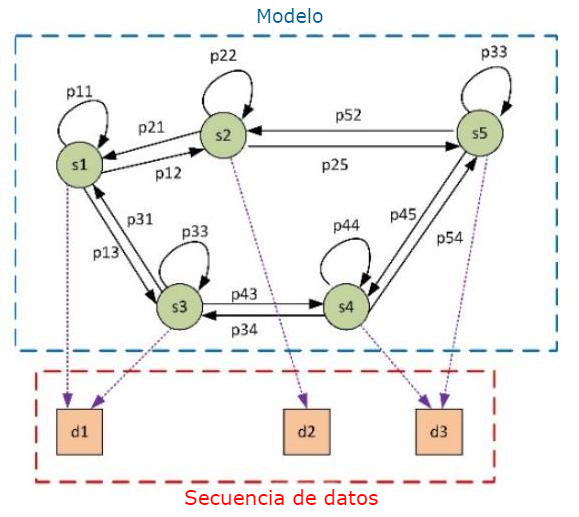
\includegraphics[max width=\textwidth]{images/2022_09_15_69d89c46b49bb93649d1g-03}

Fig. 1. Representación gráfica de un HMM\\

Los HMM, sin embargo, son inútiles para modelar ciertas actividades concurrentes, por lo que otros autores han reportado una nueva técnica denominada Conditional Random Field (CRF). Los CRF se emplean para modelar aquellas actividades que presentan acciones concurrentes o, en general, múltiples acciones que interactúan [12][13]. Además, HMM requiere un gran esfuerzo de entrenamiento para descubrir todos los estados ocultos posibles. Para resolver estos problemas, el campo aleatorio condicional (CRF) emplea probabilidades condicionales en lugar de distribuciones de probabilidad conjunta. De esa forma, se pueden modelar fácilmente actividades cuyas acciones se desarrollan en cualquier orden. A diferencia de las cadenas en HMM, CRF emplea gráficos acíclicos y permite la integración de estados ocultos condicionales (estados que dependen de observaciones pasadas y/o futuras). Los CRF, por otro lado, siguen siendo inútiles para modelar ciertos comportamientos, por lo que algunas propuestas generalizan este concepto y proponen el Skip Chain Conditional Random Field (SCCRF). SCCRF es una técnica de reconocimiento de patrones, más general que CRF, que permite modelar actividades que no son una secuencia de acciones en la naturaleza [14]. Esta técnica trata de capturar dependencias de largo alcance (cadena de salto); y puede entenderse como el producto de diferentes cadenas lineales. Sin embargo, calcular este producto es bastante pesado y complicado, por lo que esta técnica suele ser demasiado costosa desde el punto de vista computacional para implementarla en pequeños sistemas integrados. Otras propuestas emplean técnicas de descripción de mayor nivel como Emerging Patterns (EP). Para la mayoría de los autores, EP es una técnica que describe actividades como vectores de parámetros y sus valores correspondientes (ubicación, objeto, etc.) [15]. Utilizando distancias entre vectores es posible calcular y reconocer acciones desarrolladas por personas. Finalmente, otros autores han empleado con éxito técnicas secundarias como los clasificadores bayesianos [16], que identifican actividades haciendo una correspondencia entre las actividades humanas y las salidas más probables de los sensores mientras se realizan estas acciones, considerando que todos los sensores son independientes. Los árboles de decisión [17], las extensiones HMM [18] y otras tecnologías similares también se han estudiado en la literatura, aunque estas propuestas son escasas. Entre todas las tecnologías descritas, HMM no es la más poderosa. Sin embargo, encaja a la perfección con la Industria 4.0, donde las actuaciones son muy complejas pero muy estructuradas y ordenadas (según protocolos de empresa, políticas de eficiencia, etc.). Además, se requiere una retroalimentación rápida (a veces incluso en tiempo real) para garantizar que los procesos impulsados por humanos funcionen correctamente antes de que ocurra una falla crítica global. Por lo tanto, las soluciones computacionalmente costosas no son un enfoque válido, y estamos seleccionando HMM como tecnología de base principal. Para preservar su carácter liviano y, al mismo tiempo, poder modelar actividades complejas, introducimos un esquema de reconocimiento de dos fases que permite dividir acciones complejas en dos pasos más simples. 


\section{Un algoritmo de reconocimiento de patrones de dos fases}
Con el fin de (i) independizar el proceso de reconocimiento de patrones de los dispositivos de
hardware empleados para capturar información, (ii) permitir el reconocimiento de acciones
complejas y (iii) preservar el carácter liviano de los modelos seleccionados, la solución propuesta
presenta una arquitectura con tres capas diferentes (ver Figura 2).

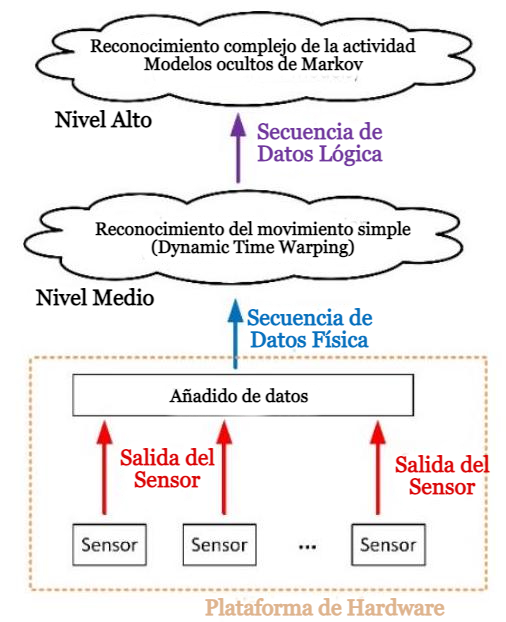
\includegraphics[max width=\textwidth]{images/2022_09_15_69d89c46b49bb93649d1g-04}

Fig. 2. Arquitectura de la solución de reconocimiento de patrones propuesta\\

La capa más baja incluye la plataforma de hardware. Los dispositivos de monitoreo como acelerómetros, teléfonos inteligentes, sensores infrarrojos, etiquetas RFID, etc., se implementan para capturar información sobre el comportamiento de las personas. Las salidas de estos dispositivos crean secuencias de datos físicos cuyo formato, rango dinámico, etc., dependen totalmente de las tecnologías de hardware seleccionadas. Estas secuencias de datos físicos luego se procesan en la capa intermedia utilizando técnicas DTW. Como resultado, para cada secuencia de datos físicos, se reconoce un movimiento o acción simple. Estas acciones simples se representan mediante un formato de datos binarios para que la solución sea lo más ligera posible. El software en este nivel debe modificarse cada vez que se actualiza la plataforma de hardware, pero las tecnologías DTW no requieren un proceso de actualización pesado, y actualizar el repositorio de patrones es suficiente para configurar el algoritmo en este nivel. Los movimientos simples reconocidos, entonces, se agrupan para crear secuencias de datos lógicos. Estas secuencias alimentan un sistema de reconocimiento de patrones de alto nivel basado en modelos ocultos de Markov. En este nivel, los componentes de software requieren un proceso de entrenamiento pesado, pero la capa intermedia hace que la plataforma de hardware y los modelos de alto nivel sean totalmente independientes. Por lo tanto, cualquier cambio en la plataforma de hardware no impone una actualización en el HMM, lo que sería extremadamente costoso desde el punto de vista computacional. Mediante el análisis de la secuencia de movimientos simples, se reconocen acciones complejas. La siguiente subsección describe en detalle las dos fases de reconocimiento de patrones propuestas.

\subsection{Reconocimiento de movimiento simple: Dynamic Time Warping}
Para reconocer gestos o movimientos simples, se selecciona una solución Dynamic Time Warping. Las tecnologías DTW cumplen con los requisitos de los componentes de software de nivel medio, ya que se adaptan muy fácilmente a las características de la plataforma de hardware subyacente y son bastante rápidas y eficientes (por lo que los pequeños dispositivos integrados pueden implementarlas). En nuestra solución, el comportamiento humano es monitoreado a través de una familia de sensores $\mathcal{S}$, que contiene $N_{s}$ componentes (1). 

$$
\mathcal{S}=\left\{s_{i}, i=1, \ldots, N_{s}\right\}
$$
Las salidas de estos sensores se muestrean periódicamente cada    $T_{s}$ segundos; obteniendo para cada instante de tiempo, t,un vector de $N_{s}$ (cada valor de cada sensor). Este vector $Y_{t}$ se llama “una muestra multidimensional”. (2) 
$$
Y_{t}=\left\{y_{t}^{i}, i=1, \ldots, N_{s}\right\}
$$
Entonces, un simple movimiento Y tendrá una duración de $T_{m}$ segundos y será descrita por la secuencia temporal de $N_{m}$ muestras multidimensionales recolectadas durante este tiempo (3). Para reconocer posteriormente los movimientos, un repositorio de patrones $\mathcal{R}$ se crea conteniendo las correspondientes secuencias temporales para cada uno de las K acciones simples para ser reconocidas (4)
$$
\begin{gathered}
Y=\left\{Y_{t}, t=1, \ldots, T_{m}\right\}=\left\{Y^{i}, i=1, \ldots, N_{m}\right\} \\
\mathcal{R}=\left\{R_{i}, i=1, \ldots, K\right\}
\end{gathered}
$$
En general, las personas realizan movimientos de manera similar pero diferente. Así, las transiciones pueden ser más lentas o más rápidas, se pueden agregar o quitar algunas acciones elementales, etc.  Por lo tanto, dada una secuencia $X$ con $N_{x}$ muestras, representando un movimiento a ser reconocido, se debe localizar el patrón $R_{i} \in \mathcal{R}$ más cerca a $X$; así que $R_{i}$ se reconoce como la acción realizada. Para ello se define una función distancia (5). Esta función de distancia se puede aplicar para calcular una matriz de costos, requerida ya que las muestras generalmente no tienen la misma longitud ni están alineadas (6).
$$
\begin{aligned}
&d: \mathcal{F} \times \mathcal{F} \rightarrow \mathbb{R}^{+}, \quad X^{i}, r_{j}^{i} \in \mathcal{F} \\
&C \in \mathbb{R}^{N_{x} \times N_{m}} C(n, m)=d\left(X^{n}, R_{j}^{m}\right)
\end{aligned}
$$
En los sensores posicionales (acelerómetros, dispositivos infrarrojos, etc.) la función de distancia se aplica directamente a las salidas de los sensores (a diferencia de, por ejemplo, los micrófonos cuyas salidas deben evaluarse en el dominio de la potencia). Aunque se pueden emplear otras funciones de distancia (la divergencia simétrica de Kullback-Leibler o la distancia de Manhattan), para este primer trabajo estamos empleando la distancia euclidiana estándar (7)

$$
d\left(X^{n}, R_{j}^{m}\right)=\sqrt{\sum_{i=1}^{N_{S}}\left(x_{i}^{n}-r_{i}^{m, j}\right)^{2}}
$$
Entonces, se define un camino de deformación $p=\left(p_{1}, p_{2}, \ldots, p_{L}\right)$ como una secuencia de pares $\left(n_{\ell}, m_{\ell}\right)$ con $\left(n_{\ell}, m_{\ell}\right) \in\left[1, N_{x}\right] \times\left[1, N_{m}\right]$ and $\ell \in[1, L]$, cumpliendo tres condiciones: (i) la condición de contorno, es decir $p_{1}=[1,1]$ y $p_{L}=\left[N_{x}, N_{m}\right]$; (ii) la condición de monotonicidad, es decir: $n_{1} \leq n_{2} \leq \cdots \leq n_{L}$ and $m_{1} \leq m_{2} \leq \cdots \leq m_{L}$; y (iii) la condición del tamaño del paso, es decir  $p_{\ell}-p_{\ell-1} \in\{(1,0),(0,1),(1,1)\}$ con $\ell \in[1, L-1]$.
Entonces, el costo total de un camino de deformación $p_{i}$ se calcula sumando todos los costes parciales o distancias (8). Con todo esto, la distancia entre dos secuencias de datos $R_{i}$ y X se define como el costo (distancia) de la ruta de pandeo óptima $p^{*}(9)$.
$$
\begin{gathered}
d_{p_{i}}\left(X, R_{j}\right)=\sum_{\ell=1}^{L} d\left(X^{n_{\ell}}, R_{j}^{m_{\ell}}\right) \\
d_{D T W}\left(X, R_{j}\right)=d_{p^{*}}\left(X, R_{j}\right)=\min \left\{d_{p_{i}}\left(X, R_{j}\right), \text { being } p_{i} \text { a warping path }\right\}
\end{gathered}
$$
Finalmente, el movimiento simple reconocido a partir de la secuencia de datos X es aquello cuyo patrón $R_{i}$  tiene la distancia más pequeña (es el más cercano) a X.
El uso de esta definición es tolerante a las variaciones de velocidad en la ejecución del movimiento, a la introducción de nuevos microgestos, etc. Además, como se puede observar, cuando se despliega una tecnología de hardware diferente, basta con actualizar el repositorio de patrones $\mathcal{R}$ para reconfigurar toda la solución de reconocimiento de patrones (ya que no se requiere capacitación). 



\subsection{Reconocimiento de acciones complejas: modelos ocultos de Markov}
El mecanismo propuesto anteriormente es muy útil para reconocer acciones simples, pero las actividades complejas involucran una gran cantidad de variables y requieren mucho más tiempo. Por lo tanto, DTW tiende a volverse impreciso y se requieren modelos probabilísticos. Entre todos los modelos existentes, HMM es el más adecuado para escenarios industriales y procesos impulsados por humanos.


De la fase anterior, se despliega el universo de posibles movimientos simples a reconocer $\mathcal{M}=\left\{m_{i}, i=1, \ldots, K\right\}$. Además, se define un universo de estados $\mathcal{U}=\left\{u_{i}, i=1, \ldots, Q\right\}$,  describiendo todos los estados que las personas pueden atravesar mientras realizan alguna de las acciones objeto de estudio. Entonces, también se considera un conjunto de observaciones $\mathcal{O}=\left\{o_{i}, i=1, \ldots, Z_{o}\right\}$ (movimientos simples reconocidos en la fase anterior), así como la secuencia de estados $V=\left\{o_{i}, i=1, \ldots, Z_{v}\right\}$ que describen la acción, como un modelado por HMM. En este caso inicial, estamos suponiendo que cada observación corresponde a un nuevo estado, por lo que  $Z_{v}=Z_{o}$ . Luego, se calculan tres matrices: (i) la matriz transitoria  A (10) que describe la probabilidad de estado $u_{j}$ siguiente el estado $u_{i}$; (ii) la matriz de observación (11) que describe la probabilidad de observación $o_{i}$ causada por el estado $u_{j}$ independientemente de $k$; y (iii) la matriz de probabilidad inicial (12).

$$
\begin{aligned}
& A=\left[a_{i, j}\right] \quad a_{i, j}=P\left(v_{k}=u_{j} \mid v_{k-1}=u_{i}\right) \\
& B=\left[b_{j}\left(o_{i}\right)\right] \quad b_{j}\left(o_{i}\right)=P\left(x_{k}=o_{i} \mid v_{k}=u_{j}\right) \\
& \Pi=\left[\pi_{i}\right] \quad \pi_{i}=P\left(v_{1}=u_{i}\right)
\end{aligned}
$$
Entonces, el HMM para que cada actividad compleja $\lambda_{i}$ sea reconocida está descrito por estos tres elementos anteriores (13).
$$
\lambda_{i}=\left\{A_{i}, B_{i}, \Pi_{\mathrm{i}}\right\}
$$
Además, se hacen dos suposiciones: (i) la suposición de Markov (14) que muestra que cualquier estado sólo depende del anterior; y (ii) el supuesto de independencia (15) que establece que cualquier secuencia de observación depende únicamente del estado actual, no de estados u observaciones anteriores.
$$
\begin{gathered}
P\left(v_{k} \mid v_{1}, \ldots, v_{k-1}\right)=P\left(v_{k} \mid v_{k-1}\right) \\
P\left(o_{k} \mid o_{1}, \ldots, o_{k-1}, v_{1}, \ldots, v_{k}\right)=P\left(o_{k} \mid v_{k}\right)
\end{gathered}
$$
Para evaluar el modelo y reconocer la actividad que realizan los usuarios, en este artículo estamos utilizando un enfoque tradicional (16). Aunque se ha demostrado que los algoritmos directos son más eficientes, para este trabajo inicial estamos implementando directamente la expresión de evaluación en su forma tradicional.
$$
\begin{gathered}
P(\mathcal{O} \mid \lambda)=\sum_{V} P(\mathcal{O} \mid V, \lambda) P(V \mid \lambda)= \\
=\sum_{V}\left(\prod_{i=1}^{z_{o}} P\left(o_{i} \mid v_{i}, \lambda\right)\right)\left(\pi_{v 1} \cdot a_{v 1 v 2} \cdot \ldots \cdot a_{v_{z v-1} v_{z v}}\right)= \\
=\sum_{v 1, v 2, . ., v_{z v}} \pi_{v 1} \cdot b_{v 1}\left(o_{1}\right) \cdot a_{v 1 v 2} \cdot b_{v 2}\left(o_{2}\right) \cdot \ldots \cdot a_{v_{z v-1} v_{z v}} \cdot b_{v z v}\left(o_{z o}\right)
\end{gathered}
$$
El proceso de aprendizaje también se implementó en su forma más sencilla. Se emplearon definiciones estadísticas para la matriz transitoria, matriz de observación y matriz de probabilidad inicial. En particular, se empleó la definición de probabilidad de Laplace para estimar estas tres matrices a partir de estadísticas sobre las actividades en estudio (17-19). El operador count$(\cdot)$ indica el número de veces que ocurre un evento.

$$
\begin{gathered}
a_{i, j}=P\left(u_{j} \mid u_{i}\right)=\frac{\operatorname{count}\left(u_{j} \text { follows } u_{i}\right)}{\operatorname{count}\left(u_{j}\right)} \\
b_{j}\left(o_{i}\right)=P\left(o_{i} \mid u_{j}\right)=\frac{\operatorname{count}\left(o_{i} \text { is observed in the state } u_{j}\right)}{\operatorname{count}\left(u_{j}\right)} \\
\pi_{i}=P\left(v_{1}=u_{i}\right)=\frac{\operatorname{count}\left(v_{1}=u_{i}\right)}{\operatorname{count}\left(v_{1}\right)}
\end{gathered}
$$

\section{Validación experimental: implementación y resultados}
Para evaluar el desempeño de la solución propuesta, se diseñó y llevó a cabo una validación experimental. Se emuló un escenario industrial en unas amplias salas de la Universidad Politécnica de Madrid. El escenario representaba una empresa tradicional que fabricaba productos hechos a mano. En particular, se emuló un pequeño fabricante de PCB (placas de circuito impreso). Para capturar información sobre el comportamiento de las personas, a los participantes se les proporcionó un guante cibernético, que incluía acelerómetros y un lector RFID [19]. Los objetos alrededor de los escenarios se identificaron con una etiqueta RFID, por lo que la plataforma de hardware propuesta puede identificar la posición de la mano (gesto) y los objetos con los que interactúan las personas. Se definió y reconoció una lista de doce actividades complejas diferentes utilizando la tecnología propuesta. La Tabla 1 describe las doce actividades definidas, incluyendo una breve descripción de las mismas.\\

Table 1. Complex activities' description\\

\begin{tabular}{|l|l|}
\hline
\multicolumn{1}{|c|}{Actividad} & \multicolumn{1}{|c|}{Descripción} \\
\hline
Dibuja los caminos del circuito & El circuito a imprimir se diseña mediante \\ &   un programa de software específico para PC. \\
\hline
Imprima el diseño del circuito usando un trazador & Usando láminas de plástico y \\ & una impresora especial llamada trazador, \\ &  se imprime el diseño del circuito. \\
\hline
Limpiar el laminado de cobre de los tableros & Usando un producto especial, todo el polvo \\ &  y las partículas se eliminan del \\ &  laminado de cobre. \\
\hline
Copie el diseño del circuito en tableros de cobre. & El diseño del circuito en la hoja de plástico \\ &  se copia en el laminado de cobre \\ &  usando una ráfaga de luz
ultravioleta. \\
\hline
Sumergir las tablas en la piscina de ácido & Para eliminar todo el cobre \\ &  no deseado, la placa impresa se \\ & sumerge en un baño de ácido. \\
\hline
Lave el cobre con un baño de disolvente. & Después del baño de ácido, \\ & la superficie de cobre restante \\ &  se lava en un baño de disolvente. \\
\hline
Alineación de capas & Los PCB se componen de varias capas; \\ & apilados y alineados durante esta fase. \\
\hline
Inspección óptica & Usando un láser, se verifica la \\ &  alineación de la capa. \\
\hline
Unir las capas exteriores con el sustrato & Usando un pegamento epoxi, se unen \\ & la capa final y la exterior del tablero. \\
\hline
Unir el tablero & La unión ocurre en una mesa \\ &  de acero pesado con abrazaderas de metal. \\
\hline
Taladre los agujeros requeridos & Los agujeros para los componentes, etc.,\\ &  se taladran en el tablero de la pila.  \\
\hline
Enchapado & En un horno, el tablero está terminado.\\
\hline
\end{tabular}\\
\newline

Dieciocho personas (18) participaron en el experimento. Se solicitó a las personas que realizaran las actividades en un número aleatorio. El orden real, así como el orden en que se reconocen las actividades, fueron almacenados por un proceso de software de supervisión. Se evaluó la tasa de éxito global para toda la solución, identificando (además,) la misma tasa para cada una de las fases existentes.
\newline

Para evaluar la mejora obtenida en comparación con soluciones similares existentes, se emplearon las mismas secuencias de datos físicos para alimentar una solución estándar de reconocimiento de patrones basada únicamente en HMM. Utilizando un software de procesamiento de datos estadísticos, se extraen algunos resultados relevantes.
\newline

La figura 4 representa la tasa media de éxito para tres casos: la solución global, la primera fase (DTW) y la segunda fase (HMM). Además, también se incluye la tasa de éxito del enfoque tradicional basado en HMM. Como puede verse, la tecnología propuesta es, globalmente, alrededor de un 9\% mejor que las técnicas tradicionales de reconocimiento de patrones basadas exclusivamente en HMM. Además, la primera fase (basada en DTW) es alrededor de un 20\% peor que la segunda fase (HMM), lo que es significativo ya que las técnicas de deformación dinámica del tiempo son más débiles de forma predeterminada.\\


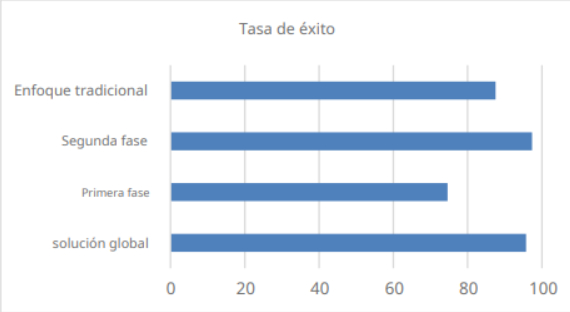
\includegraphics[max width=\textwidth]{images/2022_09_15_69d89c46b49bb93649d1g-09}

Fig. 4. Tasa media de éxito de la solución propuesta

\section{Conclusión y futuros trabajos}
En este artículo, presentamos un nuevo algoritmo de reconocimiento de patrones para integrar personas en los sistemas y procesos impulsados por humanos de la Industria 4.0. El algoritmo define actividades complejas como composiciones de movimientos simples. Las actividades complejas se reconocen utilizando Modelos ocultos de Markov y los movimientos simples se reconocen utilizando Dynamic Time Warping. 
Para permitir la implementación de este algoritmo en pequeños dispositivos embebidos, se seleccionan configuraciones ligeras. También se realiza una validación experimental, y los resultados muestran una mejora global en la tasa de éxito en torno al 9\%. Los trabajos futuros considerarán las metodologías más complejas para el procesamiento de datos y se evaluará la comparación para diferentes configuraciones del algoritmo propuesto. Además, la propuesta será analizada en diferentes escenarios. 


Agradecimientos. La investigación que ha dado lugar a estos resultados ha recibido financiación del Ministerio de Economía y Competitividad a través del proyecto SEMOLA (TEC2015-68284-R) y del Ministerio de Ciencia, Innovación y Universidades a través del proyecto VACADENA (RTC-2017-6031-2).


\section{Bibliografía}
\begin{enumerate}
  \item Bordel, B., Alcarria, R., Sánchez-de-Rivera, D., \& Robles, T. (2017, November). Protecting industry $4.0$ systems against the malicious effects of cyber-physical attacks. In International Conference on Ubiquitous Computing and Ambient Intelligence ( $\mathrm{pp}$. 161171). Springer, Cham.

  \item Bordel, B., Alcarria, R., Robles, T., \& Martín, D. (2017). Cyber-physical systems: Extending pervasive sensing from control theory to the Internet of Things. Pervasive and mobile computing, 40, 156-184.

  \item Neff, W. (2017). Work and human behavior. Routledge.

  \item Bordel, B., Alcarria, R., Martín, D., Robles, T., \& de Rivera, D. S. (2017). Selfconfiguration in humanized cyber-physical systems. Journal of Ambient Intelligence and Humanized Computing, 8(4), 485-496.

  \item Bordel, B., de Rivera, D. S., Sánchez-Picot, Á., \& Robles, T. (2016). Physical processes control in industry 4.0-based systems: A focus on cyber-physical systems. In Ubiquitous Computing and Ambient Intelligence (pp. 257-262). Springer, Cham.

  \item Pal, S. K., \& Wang, P. P. (2017). Genetic algorithms for pattern recognition. CRC press.

  \item Müller, M. (2007). Dynamic time warping. Information retrieval for music and motion, 69-84.

  \item Eddy, S. R. (1996). Hidden markov models. Current opinion in structural biology, 6(3), 361-365.

  \item Kim, E., Helal, S., \& Cook, D. (2010). Human activity recognition and pattern discovery. IEEE Pervasive Computing/IEEE Computer Society [and] IEEE Communications Society, $9(1), 48 .$

  \item Li, Z., Wei, Z., Yue, Y., Wang, H., Jia, W., Burke, L. E., ... \& Sun, M. (2015). An adaptive hidden markov model for activity recognition based on a wearable multi-sensor device. Journal of medical systems, $39(5), 57 .$

  \item Ordonez, F. J., Englebienne, G., De Toledo, P., Van Kasteren, T., Sanchis, A., \& Krose, B. (2014). In-home activity recognition: Bayesian inference for hidden Markov models. IEEE Pervasive Computing, 13(3), 67-75.

  \item Zhan, K., Faux, S., \& Ramos, F. (2015). Multi-scale conditional random fields for firstperson activity recognition on elders and disabled patients. Pervasive and Mobile Computing, 16, 251-267.

  \item Liu, A. A., Nie, W. Z., Su, Y. T., Ma, L., Hao, T., \& Yang, Z. X. (2015). Coupled hidden conditional random fields for RGB-D human action recognition. Signal Processing, 112, 74-82.

  \item Liu, J., Huang, M., \& Zhu, X. (2010, July). Recognizing biomedical named entities using skip-chain conditional random fields. In Proceedings of the 2010 Workshop on Biomedical Natural Language Processing (pp. 10-18). Association for Computational Linguistics.

  \item Gu, T., Wu, Z., Tao, X., Pung, H. K., \& Lu, J. (2009, March). epsicar: An emerging patterns based approach to sequential, interleaved and concurrent activity recognition. In Pervasive Computing and Communications, 2009. PerCom 2009. IEEE International Conference on (pp. 1-9). IEEE.

  \item Hu, B. G. (2014). What are the differences between Bayesian classifiers and mutualinformation classifiers? IEEE Trans. Neural Netw. Learning Syst., 25(2), 249-264.

  \item Wang, X., Liu, X., Pedrycz, W., \& Zhang, L. (2015). Fuzzy rule based decision trees. Pattern Recognition, 48(1), 50-59.

  \item Davis, M. H. (2018). Markov models \& optimization. Routledge.

  \item Bordel Sánchez, B., Alcarria, R., Martín, D., \& Robles, T. (2015). TF4SM: a framework for developing traceability solutions in small manufacturing companies. Sensors, 15(11), 29478-29510.

\end{enumerate}

\end{document}